\subsection{Sprint Backlog}
En este documento se planifica todo el ciclo de vida de desarrollo de cada módulo del sistema, integrando un ID, el nombre del módulo, la fecha de incio y fin del proceso y un responsable de ese proceso.
\subsubsection{Primer Sprint}
\begin{figure}[!h]
	\centering
	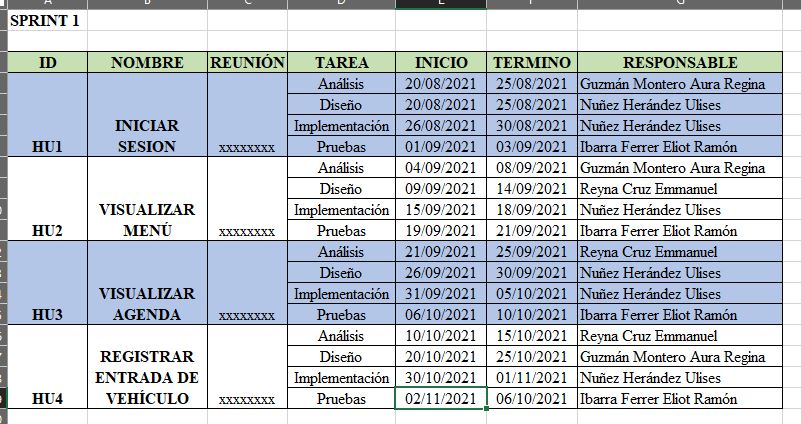
\includegraphics[width=1\textwidth]{./sprintBacklog/imagenes/sprint1}
	\caption{Primer Sprint - Sprint Backlog}
	\label{fig:Primer Sprint - Sprint Backlog}
\end{figure}
\clearpage
\subsubsection{Segundo Sprint}
\begin{figure}[!h]
	\centering
	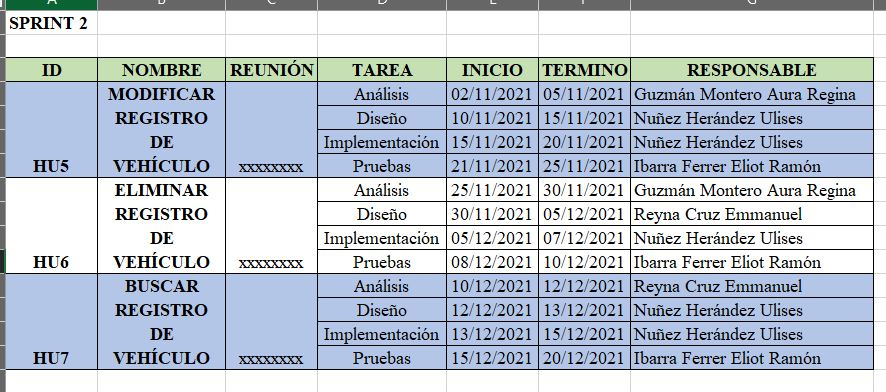
\includegraphics[width=1\textwidth]{./sprintBacklog/imagenes/sprint2}
	\caption{Segundo Sprint - Sprint Backlog}
	\label{fig:egundo Sprint - Sprint Backlog}
\end{figure}